% Teilauswertung X

\section{Absorption und Dispersion einer Jodlinie}


\begin{figure}[h]
    \centering
    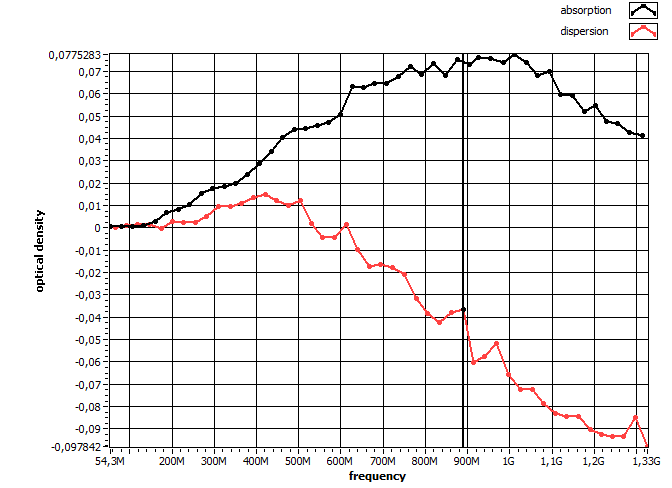
\includegraphics[width=0.95\textwidth]{Bilder/Jodlinie/Gruppe32020Iododgraph1 Kopie.png}
    \caption[Iodlinie]{Iodlinie}
\end{figure}

\subsection{Nachprüfen der Absorption}

Zur Nachprüfung des Berechneten Absorptionssignals wurden bei drei Frequenzen manuell eine Messung mit und ohne Probe durchgeführt.

Fehlerrechnung für OD!!
\begin{table}[h]
    \centering
    \begin{tabular}{c|cc|c}
        $\omega_m$/MHz & $\Delta U_{Ref}$ / mV & $\Delta U_{Probe}$ / mV & OD \\ \hline
        79,7 & $128 \pm 4$ & $130 \pm 4$ & $-6,73 \cdot 10^{-3}$ \\
        491,9 & $268 \pm 4$ & $270 \pm 4$ & $-3,23 \cdot 10^{-3}$ \\
        989,1 & $283 \pm 4$ & $320 \pm 4$ & $-0,0534$ \\
    \end{tabular}
    \caption[short]{title}
\end{table}